\chapter{Architecture}
\label{cap:cap03}

Architectural design is strongly tied down by OpenFlow 1.3 required and optional elements. With the architecture description, we do not intend to repeat the specification. Thus, elements described in the next sections are an specific and conceptual point of view of each software switch component. 

The OpenFlow switch implementation is a fork from the OpenFlow 1.1 reference switch. We choose this implementation as a starting point for our work because of the simpler code base, when compared to other switch implementations discussed in section \ref{cap:cap02}. Although simple, the only documentation available to understand the reference switch was the OpenFlow specification. For this reason, the definition of the architectural design started from the extraction of the previous software architecture. 

Firstly, through a simple reverse software engineering process \cite{Sommerville:2001:SE:375369}, we analyzed the code and listed the switch core components. Next, we identified missing components from the OpenFlow 1.3 specification. After these steps, we found that block structures suggest the application of a bottom-up design \cite{vonMayrhauser:1990:SEM:79005}. In this approach, the basic set of foundational modules and their interrelationships are the foundation for the final architecture. Following these concepts, we came up with the final design for the OpenFlow 1.3 software switch.

In the Figure \ref{fig:switcharq} we show the software switch architecture. The most important block is the Datapath. It consists of OpenFlow internal elements such as Flow, Meter and Group Tables, and a Packet Parser as well. The other three blocks operate on different levels along with the Datapath. From the top level, the blocks Datapath, Marshaling/Unmarshaling library and Communication Channel are part of the OpenFlow message layer. Below, Ports and Datapath form the network packets layer, where packets arrive, are processed and usually sent back for the network.\footnote{Some instructions, actions and even an empty table may cause a packet drop in the Datapath.} Except for the special case of the \textit{Packet In} message, in which packets can be sent for the controller, these two layers do not interact. In Figure \ref{fig:switcharq}, dotted lines illustrate some possible paths a network packet can travel between the Ports and the Datapath. Solid lines denote the OpenFlow messages traveling in the OpenFlow message layer. Arrows mean the direction packets and OpenFlow messages can take across the switch components. In this chapter, we present each software switch component individually, detailing each block roles and interactions with other elements.

\begin{figure}[H]
\centering
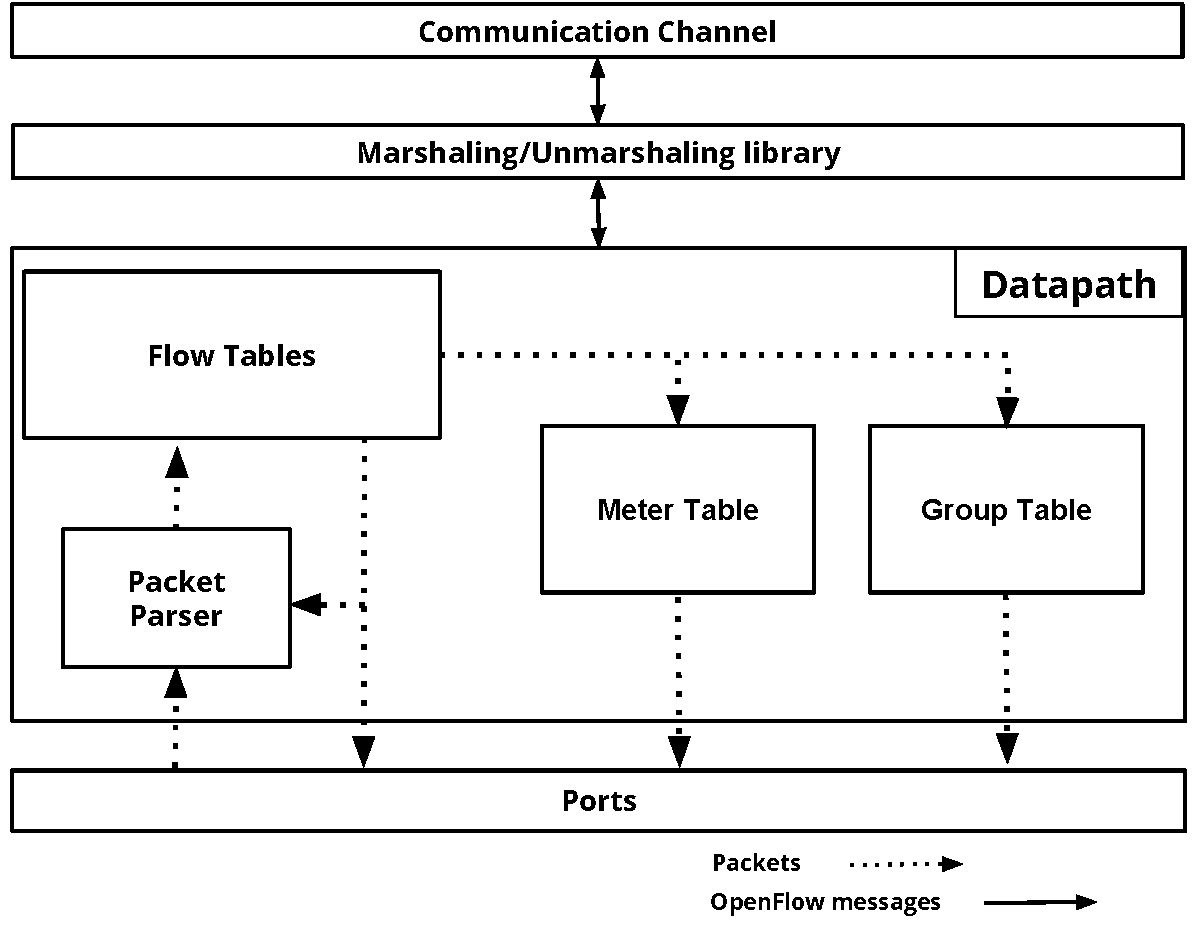
\includegraphics[height=12cm,width=\textwidth,keepaspectratio]{cap3/switcharq.pdf}
\caption{Software switch architecture}
\label{fig:switcharq}
\end{figure}

	\section{Ports}

	OpenFlow ports are the entrance and exit doors for  network packets of the OpenFlow switch pipeline. A software switch instance running on a machine may use their physical or virtual interfaces as port elements. Physical port elements can take control over Ethernet or WiFi interfaces, allowing the creation of real network topologies. Although limited by the speed of the software switch, the possibility to create a low cost testbed enriches the experience of users developing and testing OpenFlow applications.     

	Ports functions on the switch are not limited to the task of send and receive packets. There is a set of responsibilities associated with the OpenFlow protocol and the pipeline. Functionalities are:

	\begin{itemize}

	\item OpenFlow enables some level of control over a port behavior. A port modification message permits the configuration of the port state. Ports can be administratively set to drop all received or forwarded packets, forbid the generation of \textit{Packet In} messages from arriving packets, and brought down. Ports elements should handle these messages and change the port behavior according to the configuration sent.

	\item OpenFlow Ports keep the current state of the physical link. This information is not configurable by an OpenFlow controller, but the switch should inform the control plane about link state changes. Ports monitor the state of the port link and update the information according to changes.

	\item Packets encapsulated in \textit{Packet In} usually have only the header sent within the message. A buffer stores the packet, while waiting for the controller decision after the \textit{Packet In}. Ports elements store these packets and resend them for further processing.

	\item An OpenFlow controller can ask the switch about a port description. The software switch element retrieves information such as current and max operating speeds from the interfaces of the machine and stores it. On a port description request, the element handles the message and sends the required information to the control plane.

	\item Queues creation are not part of the OpenFlow protocol. However, OpenFlow can configure port queues, created by whichever mechanism, to be associated with a switch port. Ports are responsible for handling queue association and configuration.  

	\item Ports must update port and queue packet counters.           
	\end{itemize}

	\section{Packet Parser}

	Before entering the software switch OpenFlow pipeline, packet protocol fields are extracted by the Packet Parser element. Parsing packets was a formally defined task until OpenFlow 1.1. The main reason to define how packets should be parsed is to guarantee parsing consistency, but it limits switch designers and demands algorithm updates for each new protocol addition. For this reason, further specifications removed how packets should be parsed and match fields are now defined only logically.

	A Packet Parser element converts extracted protocol fields of a packet to an internal flow entry format. Two scenarios may trigger this function:   

	\begin{itemize}

	\item A network packet enters the switch through one of its ports.    

	\item  If the packet was modified by an action and is resubmitted for the pipeline, or sent to a table ahead by a \textit{Go To Table} instruction, packet revalidation is required. Hence the packet is processed by the Packet Parser again. In Figure \ref{fig:switcharq}, after passing by the Flow Tables, there is an arrow representing packet return to the Packet Parser.        

	\end{itemize}

	Further OpenFlow extensions, supporting new protocols, directly affect the packet parsing. Modifications are required in order to add new match fields for the Packet Parser. Therefore, a flexible and extensible Packet Parser element is desirable.  

	\section{Flow Tables}

	Flow Tables are the heart of an OpenFlow switch architecture. They are the elements where flow entries are stored and the OpenFlow pipeline starts. Although the use of multiple flow tables is optional - the specification mandates at least one table - its implementation is recommended, as even simple applications can not scale in switches with only one Flow Table \cite{tableExplosion}.  
	
	Flow Tables roles in the software switch are listed below.

	\begin{itemize}

    \item In case of nonexistence of a table miss flow entry, Flow Tables have to implement some default action for not matched packets. Currently, the default action is drop the packets. 

	\item Handle \textit{Flow Mod} messages sent by the controller. These messages may add or delete flow entries, or change the instruction set from currently installed flows.  

	\item Flow Tables must be able to have their capabilities reconfigured by a controller. These table features can express the table supported properties. The instructions' type and the match fields allowed in the table are examples of properties. Also, some fields show relevant information for an OpenFlow application. For instance, the table identifier value is an information required to add a new flow, and the max number of flow entries should be considered to avoid scalability problems.           

    \item A Packet look up must be performed upon the receiving of a packet. The operation looks for a flow table entry that matches the packet. In the case of a match, the switch executes the instruction set associated with the flow entry. This is the most common activity in Flow Tables.   
    
    \item Keep table statistics about the number of active flow entries, number of look ups and matched packets.  

	\end{itemize}

	\section{Group Table}

	Group Table empowers OpenFlow forwarding options. Packets reach the Group Table after matching a flow entry containing a group action, in one of the Flow Tables. 
	
	Group entries are stored into the Group Table. Each group entry contains an identifier, a type, counters and action buckets. Action buckets are an ordered list of action sets to be executed according to the group type. Figure \ref{fig:grouptable} represents a group table filled with groups of All, Indirect and Fast Failover types. The layout of the specific group types is important, because it defines Group Table attributions, as shown by the responsibilities listed here.
	
	\begin{figure}[H]
    \centering
    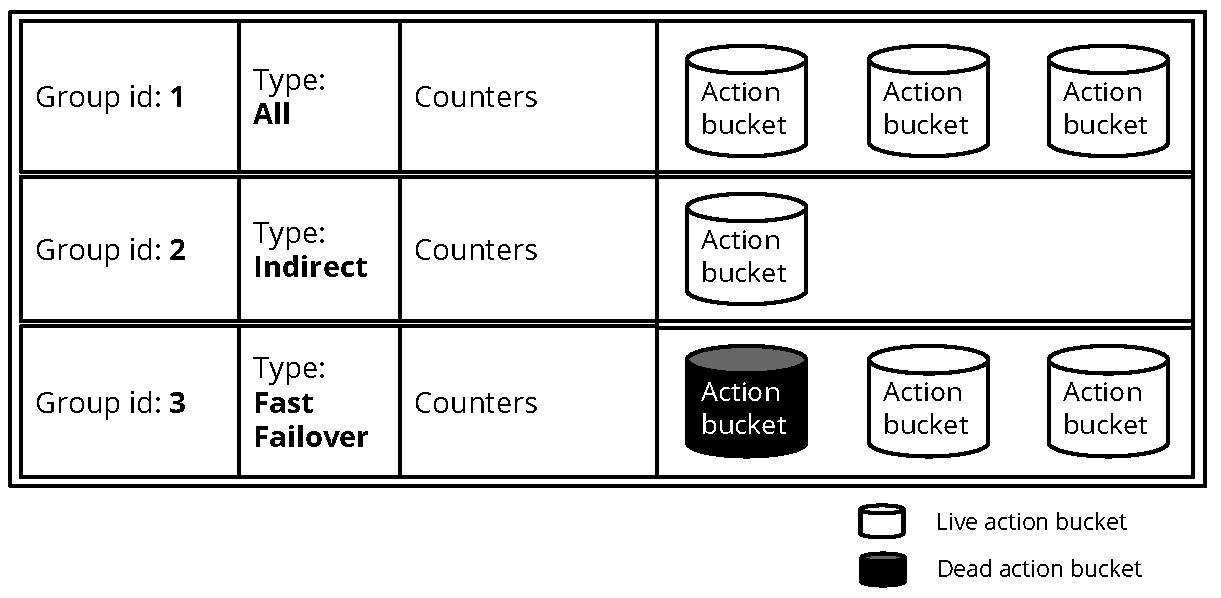
\includegraphics[height=7cm,width=\textwidth,keepaspectratio]{cap3/GroupTable.pdf}
    \caption{Group Table internals}
    \label{fig:grouptable}
    \end{figure}

	\begin{itemize}
	
	\item The Group Table have to guarantee group type restrictions. For instance, indirect groups support only one action bucket. 

	\item The Group Table must handle modification messages and perform consistency checks in the case of group chaining. Chained groups point to other groups and may cause loops that should be avoided by the element.  

	\item Fast failover groups require monitoring switch ports and group buckets for state changes. For this reason the Group Table is responsible for checking bucket liveness when choosing the first live bucket.

	\item A Group Table that supports the select group type has to implement a schedule discipline algorithm to choose which bucket will be applied to the packet.

	\end{itemize}

	\section{Meter Table}
	\label{sec:MeterTable}

    The Meter Table is an element to perform simple QoS operations. Per-flow meters are attached to flow entries through the \textit{Meter} instruction. A meter entry is composed by a meter id, counters and meter bands. The QoS operations to apply are defined by the meter bands. A meter band must have a type and rate value, which is the boundary to apply the action determined by the type. Figure \ref{fig:metertable} illustrates the internals of a Meter Table, with two meter band types.   

    \begin{figure}[H]
    \centering
    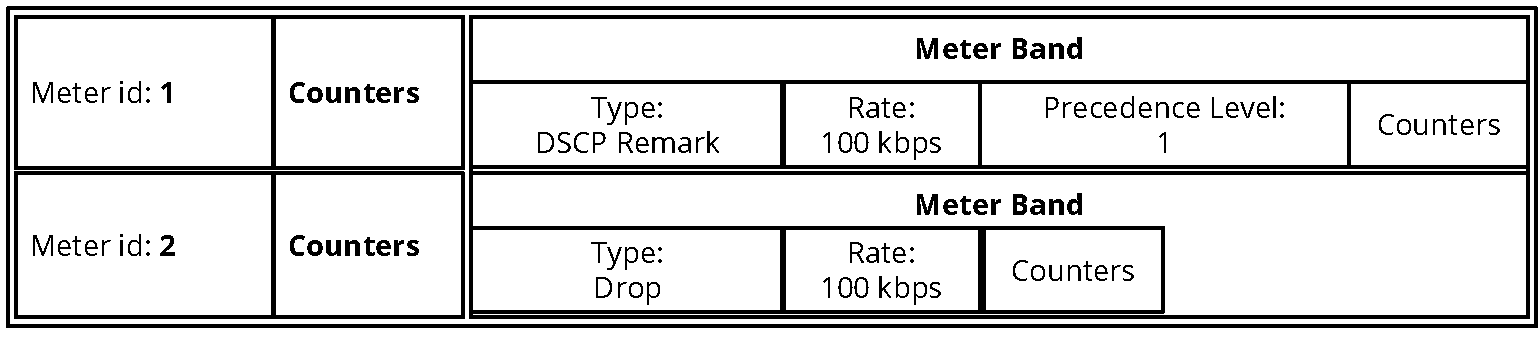
\includegraphics[height=7cm,width=\textwidth,keepaspectratio]{cap3/MeterTable.pdf}
    \caption{Meter Table internals}
    \label{fig:metertable}
    \end{figure}

    Meter Table responsibilities include:

    \begin{itemize}
    
    \item Creation, destruction and modification of meter entries.
    
    \item Matched packets, from flows pointing to the Meter Table, rate measurement. 
    
    \item Keep and update counters for statistics of packets processed by an entry.
    
    \item Process the packets according to band operation. A Drop meter band type discards the packets and the DSCP remark changes the IP packet drop precedence. 
    
    \end{itemize}

    \section{Marshaling/Unmarshaling library}
    \label{(un)pack}
    OpenFlow messages defined by the specification follow a proper format for transmission in the network. Messages are 8-byte aligned, so there may be insertion of padding fields to follow this alignment rule. Another requirement for the message format is the byte order. The preferred format for packets sent through the network is the network byte order \cite{rfc1700}. As OpenFlow messages are sent over IP networks, their messages should be assembled following the Big-Endian format.
    
    The architectures of machine's processor may operate on different byte-endianness. For instance, Intel processors use the Little-Endian byte order \cite{little-endian}. So, in order to handle and assemble OpenFlow messages, conversion is required for non Big-Endian architectures.     
    
    For the mentioned reasons, a library which abstracts byte-endianness and adds any required bytes to ensure right message format is required. A Marshaling/Unmarshaling library is not an element defined by OpenFlow specification. Its main function is the translation of OpenFlow messages from the network format to an internal format and vice-versa. The library responsibilities are the following:
    
    \begin{itemize}
    
    \item Every OpenFlow message must have a function that packs and unpacks it. Pack is the function which converts internal structures into network format. While unpack turns received messages into an internal structure.
    
        \subitem - When packing, the library has to add any necessary padding bytes.
        \subitem - On packing, the message should be assembled in network byte-order.
        \subitem - On unpacking, the library must translate the message fields to the switch host architecture byte-order.
    
    \item Some handling of OpenFlow message errors is done in this level. The library must raise errors for messages with wrong length or bad arguments. 
    
    \end{itemize}

    \section{Communication Channel}	

    The OpenFlow software switch communicates with controllers through the Communication Channel. This element connects with the Datapath and the controller and acts as a proxy between them. This element exists because the implementation of the communication channel is not defined by the specification. Since the message format is respected, implementations are free to choose the connection protocol. For instance, when security for the channel is a requirement, a protocol like TLS should be used to encrypt the messages. 
    
    In the software switch, the Communication Channel roles are:
    
    \begin{itemize}
    
    \item The Communication Channel must establish a TCP connection with the switch and the controller.
    
    \item Connection setup is a Communication Channel responsibility. After a TCP connection, the switch negotiates the protocol version with the controller. This process, known as handshake, is managed by the Communication Channel. 
    
    \item The channel may use multiple connections with a single controller at the same time. These connections can be used to send OpenFlow in parallel or to create specific channels for some message types.
    
    \item A Communication Channel is responsible for opening connections to enable switch communication with more than one OpenFlow controller. 
    
    \end{itemize}
    
    
    